\documentclass{article}
\usepackage[utf8]{inputenc}
\title{\Large  Physics 21: Spring 2021\\ \quad \\
Assignment 2}
\author{\textbf{Shubh Agrawal} \qquad
\normalsize{Class of 2022}}
\date{\today}
\usepackage[a4paper,top=2cm, left=1cm,width=14cm,bottom=2cm,right=1cm]{geometry}
\usepackage[final]{pdfpages}
\usepackage{amsthm, amsmath, amssymb, tipa, graphicx, caption, subcaption, float, fancyhdr, graphics, verbatim, cancel, hyperref}

\pagestyle{fancy}
\lhead{Physics 21}
\rhead{Assignment 2}
\chead{Shubh Agrawal}

\newcommand{\RR}{\mathbb{R}}
\newcommand{\NN}{\mathbb{N}}
\newcommand{\ZZ}{\mathbb{Z}} 
\newcommand{\la}{\langle}
\newcommand{\ra}{\rangle}
\newcommand{\dd}{\partial}

\setlength{\parindent}{0pt}

%\includepdf[pages=-,pagecommand={}, width=.90\textwidth]{main.pdf}

\begin{document}

\maketitle

\section{Part I: Introduction to FFt}
\subsection{Consistency of the Fourier transform definition}
Referring to the assignment description, equations 2 and 3 give us, with $f_k = \frac{k}{L}$:
$$h(x) = \sum_{k=-\infty}^{\infty} \widetilde{h}_k(x) \exp(2\pi i f_k x)
\qquad \qquad\qquad\qquad\qquad \widetilde{h}_k(x)= \frac{1}{L} \int_0^L h(x) \exp(2\pi i f_k x) dx$$

Inserting the latter into the former gives us:
\begin{align*}
h(x) &= \sum_{k=-\infty}^{\infty} \widetilde{h}_k(x) \exp(2\pi i f_k x) 
\\
&= \sum_{k=-\infty}^{\infty} \Big( \frac{1}{L} \int_0^L h(x') \exp(2\pi i f_k x') dx' \Big) \exp(2\pi i f_k x)
\\
&= \frac{1}{L} \int_0^L dx' \, h(x') \sum_{k=-\infty}^{\infty} \exp(2\pi i f_k (x'-x))  & \text{using } \sum_{k=-\infty}^{\infty} \exp(i 2\pi kx /L) = \sum_{n=-\infty}^{\infty} \delta(x/L - n)
\\
&= \frac{1}{L} \int_0^L dx' \, h(x') \sum_{n=-\infty}^{\infty} \delta((x'-x)/L - n)  & \text{with } f_k = \frac{k}{L} \text{ and } x \leftarrow x'-x
\\
&= \frac{1}{L} \frac{1}{1 / |L|} \int_0^L dx' \, h(x') \sum_{n=-\infty}^{\infty} \delta(x'-x-nL)  & \text{using } \delta(a x) = \frac{1}{|a|} \delta(x)
\\
&= \sum_{n=-\infty}^{\infty} \int_0^L dx' \, h(x') \delta(x'-(x+nL)) 
\end{align*}
In this integral, we must have some $n\in \mathrm{Z}$, such that $0 < x+nL < L$. We also note that there is only one such $n$, as the integral is over a range of size $L$, and each step in $n$ increases $x+nL$ by $L$. Thus, using the delta function property that $\int_{I} f(x) \delta(x-a) = a$ if $a\in I$, or $= 0$ if $a\notin I$, we get, with $0 < x+n'L < L$:
\begin{align*}
h(x) &= \sum_{n=-\infty}^{\infty} \int_0^L dx' \, h(x') \delta(x'-(x+nL)) = 0 + h(x' = x+n'L) = h(x+n'L) = h(x)
\end{align*}
as $h$ is a periodic function with period $L$, and $n'$ is an integer. Thus, we get this identity that shows our definition is self-consistent, as required.

\subsection{Completeness of Fourier Transform}
We want to show that for any values of $A, \varphi$, there exist some complex $a, b$ such that $A \sin(2\pi x / L + \varphi) = a \exp(-2\pi i x / L) + b \exp(2\pi i x / L)$. As $e^{i\theta} = \cos(\theta) + i \sin(\theta)$, we get:
\begin{align*}
a \exp(-2\pi i x / L) + b \exp(2\pi i x / L) &= a (\cos(2\pi x / L) + i \sin(2\pi x / L)) +  b (\cos(-2\pi x / L) + i \sin(-2\pi x / L))
\\
&= a \cos(2\pi x / L) + i a \sin(2\pi x / L)) +  b \cos(2\pi x / L) - i b \sin(2\pi x / L))
\\
&= (a + b) \cos(2\pi x / L) + i (a - b) \sin(2\pi x / L) 
\end{align*}
We want this value to be $A \sin(2\pi x / L + \varphi)$ for all $x$. As $\sin(A+B) = \sin A \cos B + \sin B \cos A$, we write $A \sin(2\pi x / L + \varphi) = A (\sin(2\pi x / L) \cos \varphi + \cos(2\pi x / L) \sin \varphi)$. Comparing, we write: $A \sin(2\pi x / L) \cos \varphi + A\cos(2\pi x / L) \sin \varphi = i (a - b) \sin(2\pi x / L) + (a + b) \cos(2\pi x / L)$. 

So, $A\cos\varphi = i (a-b)$ and $A\sin\varphi = a+b$. Then, $A^2\cos^2\varphi + A^2 \sin^2\varphi = A^2 \times 1 = A^2 = i^2 (a-b)^2 + (a+b)^2 = -a^2 +2ab -b^2 + a^2 + 2ab + b^2 = 4ab$. We note that as $a+b$ and $a-b$ must be purely real or purely imaginary respectively, we must have that $a$ and $b$ are complex conjugates of each other. 

Take $a = \alpha + i \beta$ and $b = \alpha - i \beta$. Then, $A\cos \varphi = i (a - b) = i (\alpha + i \beta - \alpha + i \beta) = - 2\beta$. Also, $A\sin\phi = a+b = \alpha + i \beta + \alpha - i \beta = 2 \alpha$. Then, $4ab = 4 (\alpha + i \beta) (\alpha - i \beta) = 4 (\alpha^2 - i^2 \beta^2) = 4 \alpha^2 + 4 \beta^2 = (2\alpha)^2 + (-2\beta)^2 = A^2 \sin^2\varphi + A^2 \cos^2\varphi = A^2 \times 1 = A^2$, as required. Thus, $\alpha = \frac{A}{2}\sin\varphi, \beta = -\frac{A}{2}\cos\varphi$.

Thus, we have $a = \frac{A}{2}(\sin\varphi - i\cos\varphi)$ and $b = \frac{A}{2}(\sin\varphi + i\cos\varphi)$. These coefficients satisfy $A \sin(2\pi x / L + \varphi) = a \exp(-2\pi i x / L) + b \exp(2\pi i x / L)$, for arbitrary coefficients, as needed. 

\subsection{Positive and negative frequency coefficients}
Using equation 3,
\begin{align*}
\widetilde{h}_k(x)^* &= (\frac{1}{L} \int_0^L h(x) \exp(2\pi i f_k x) dx)^* = \frac{1}{L^*} \int_0^L h(x)^* \exp(2\pi i f_k x)^* dx 
\\
&= \frac{1}{L} \int_0^L h(x) \exp(-2\pi i k x / L) dx = \frac{1}{L} \int_0^L h(x) \exp(2\pi i (-k/L) x)^* dx & \text{as $h(x)$ is real}
\\
&= \frac{1}{L} \int_0^L h(x) \exp(-2\pi i f_{-k} x) dx = \widetilde{h}_{-k}(x)
\end{align*}
Thus, $\widetilde{h}_{-k}(x) = \widetilde{h}_{k}(x)*$ as needed.

\subsection{Convolution}
We attempt to prove equation 10. We write:
\begin{align*}
H(x) &= h^{(1)}(x) h^{(2)}(x) = \sum_{k_1=-\infty}^{\infty} \widetilde{h}_{k_1}(x) \exp(2\pi i f_{k_1} x) \sum_{k_2=-\infty}^{\infty} \widetilde{h}_{k_2}(x) \exp(2\pi i f_{k_2} x) 
\\
&= \sum_{k_1, k_2=-\infty}^{\infty} \widetilde{h}_{k_1}(x) \widetilde{h}_{k_2}(x) \exp(2\pi i (f_{k_1} + f_{k_2}) x)
\end{align*}
Setting this equal to Fourier transform series of $H(x)$,
\begin{align*}
H(x) &= \sum_{k=-\infty}^{\infty} \widetilde{H}_{k}(x) \exp(2\pi i f_k x) = \sum_{k_1, k_2=-\infty}^{\infty} \widetilde{h}_{k_1}(x) \widetilde{h}_{k_2}(x) \exp(2\pi i (f_{k_1} + f_{k_2}) x)
\\
&= \sum_{k_2=-\infty}^{\infty} \Big(\sum_{k_1=-\infty}^{\infty} \widetilde{h}_{k_1}(x) \widetilde{h}_{k_2}(x)\Big) \exp(2\pi i (f_{k_1} + f_{k_2}) x)
\end{align*}
This implies $f_{k_1} + f_{k_2} = f_{k}$, or $k = k_1 + k_2$. To get the form of equation 10, we set the coefficient in either series the same, and set $k_1 \leftarrow k$, and $k_2 \leftarrow k-k'$ (to ensure $k = k_1 + k_2$). This gives us $\widetilde{H}_{k}(x) = \sum_{k'=-\infty}^{\infty} \widetilde{h}_{k'}(x) \widetilde{h}_{k - k'}(x)$, as needed.

The important note here is that multiplication in the time-space is an equivalent operation as convolution in the frequency-space (Fourier transform of time-space). Graphically speaking, a convolution is the moving average of two functions: for the two inputs to the convolution, we invert (reflect about $y$-axis) the first function and shift it by the value $k$ and integrate the product of the result and the second function over all real inputs. 

For the exercise that demonstrates a convolution of two functions, we take $\widetilde{h}_{k}(x) = k$ and $\widetilde{h}_{k}(x) =\delta_{k, 10}$. Then, using the convolution $\widetilde{H}_{k} = \sum_{k'=-\infty}^{\infty} \widetilde{h}_{k'} \widetilde{h}_{k - k'} = \sum_{k'=-\infty}^{\infty} k' \delta_{k-k',10} = 0 + 1\times k-10 = k-10$. So, the graph of $\widetilde{H}_{k}$ as a function of $k$ is a straight line with $y$-intercept -10. $\widetilde{H}_{k}$ is a constant function of $x$. \texttt{Mathematica} plot for $\widetilde{H}_{k}$ shown in Fig. \ref{fig:convolution}.

\begin{figure}[h!]
\centering
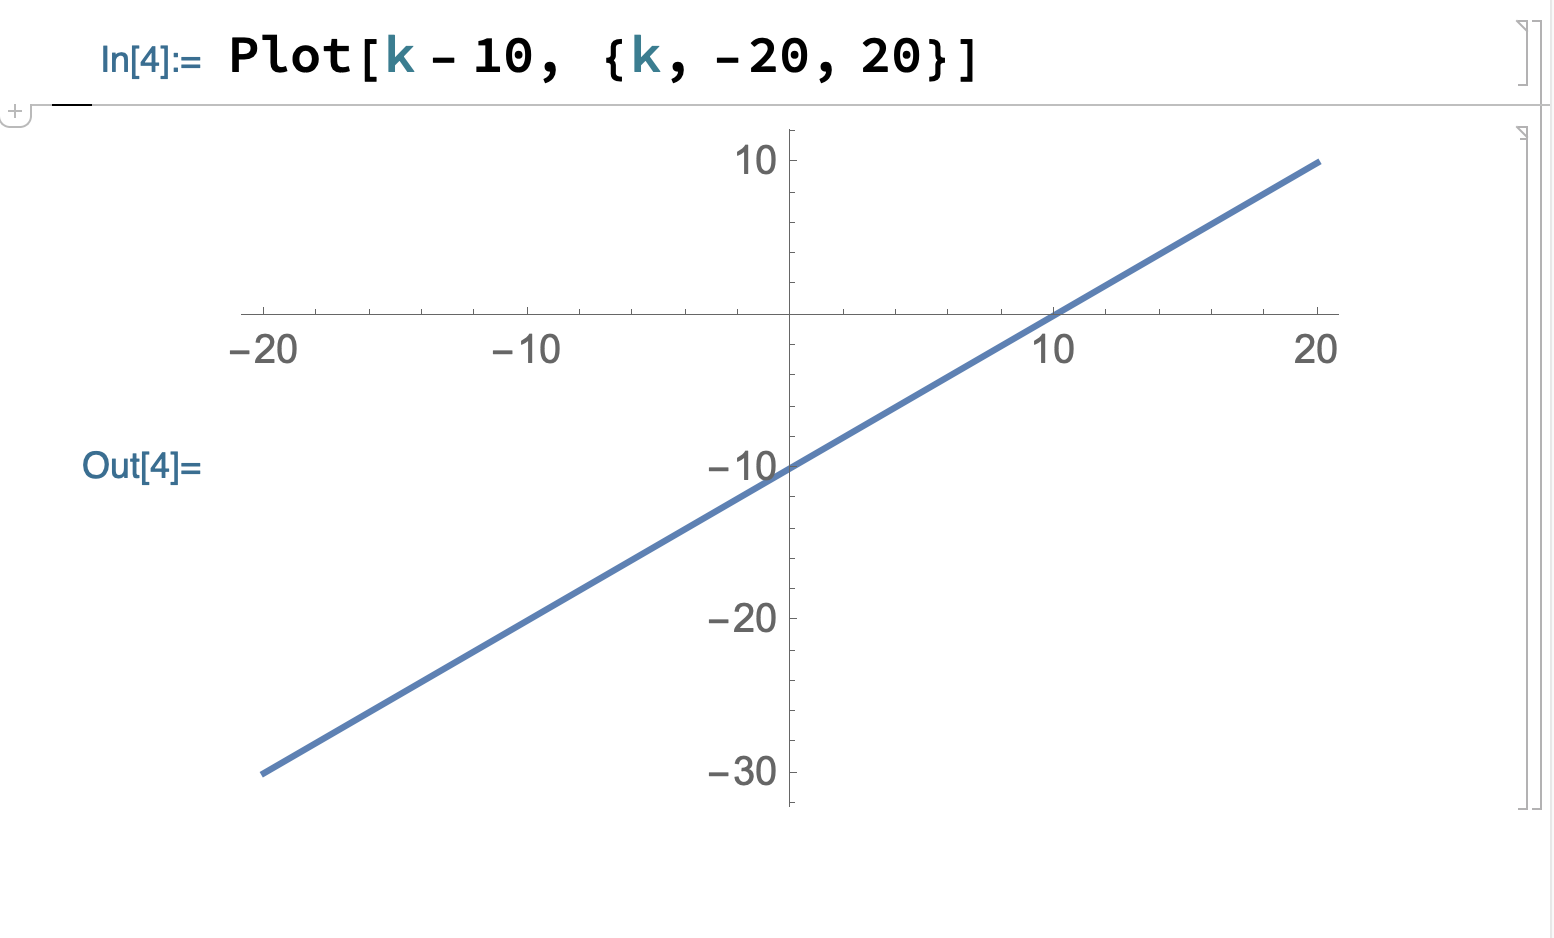
\includegraphics[width=0.75\textwidth]{plots/convolution.png}
\caption{\label{fig:convolution}  }
\end{figure}

\subsection{FFT in Python}

Analytically, the Fourier transform of a cosine function $\cos(2\pi f t)$ is a delta function at the frequency $f$ of the function. For our case $C+A\cos(2\pi f t + \phi)$, we also have a constant offset signal $C$, which will give a component of frequency 0. Thus, we expect to see three sharp peaks at $-f, 0,$ and $f$.

I created a cosine signal with $C = 5$, $A = 2$ , $f = 1$, $\phi = 1$ as seen in Fig. \ref{fig:cosine_signal}. Running our \texttt{scipy} FFT code, we get Fig. \ref{fig:cosine_fft} which has sharp peaks at $-f = -1, 0,$ and $f = 1$ as expected. Applying the inverse transform, we get the same data back again as seen in Fig. \ref{fig:cosine_inverse}.

\begin{figure}[h!]
\centering
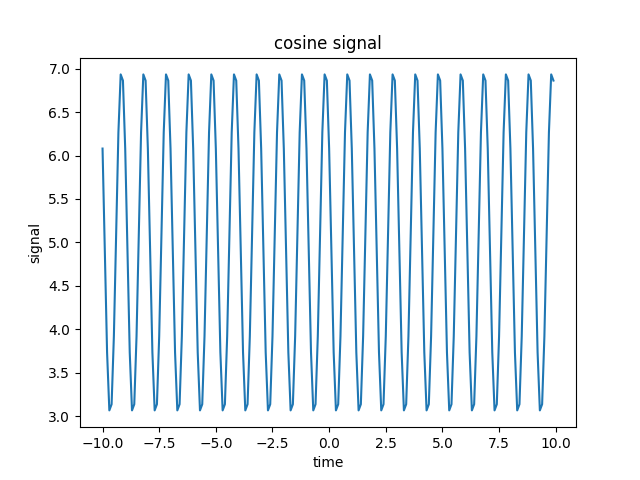
\includegraphics[width=0.75\textwidth]{plots/cosine_signal.png}
\caption{\label{fig:cosine_signal}  }
\end{figure}

\begin{figure}[h!]
\centering
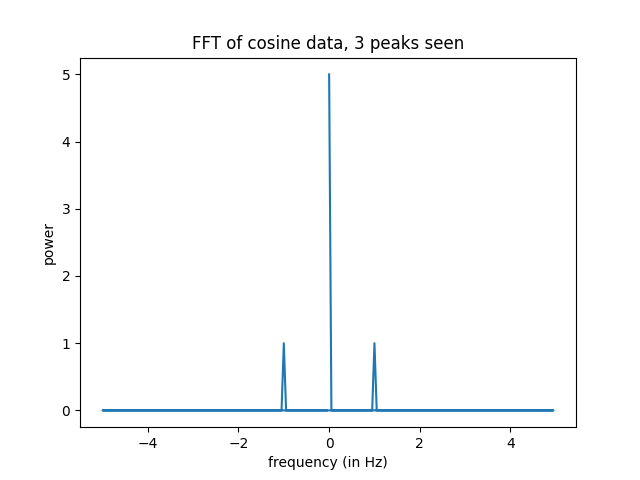
\includegraphics[width=0.75\textwidth]{plots/cosine_fft.png}
\caption{\label{fig:cosine_fft}  }
\end{figure}

\begin{figure}[h!]
\centering
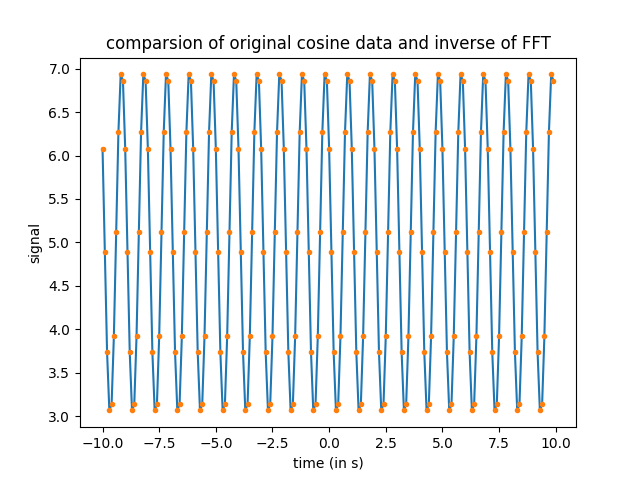
\includegraphics[width=0.75\textwidth]{plots/cosine_inverse.png}
\caption{\label{fig:cosine_inverse}  }
\end{figure}

Analytically, the Fourier transform of a Gaussian function is another Gaussian function centered at 0. Thus, we expect to see a Gaussian peak centered at 0 in frequency space.

I created a Gaussian signal with $A = 5$, $B = 50$, $L = 1$ as seen in Fig. \ref{fig:gauss_signal}. Running our \texttt{scipy} FFT code, we get Fig. \ref{fig:gauss_fft} which has a Gaussian peak centered at 0 as expected. Applying the inverse transform, we get the same data back again as seen in Fig. \ref{fig:gauss_inverse}.

\begin{figure}[h!]
\centering
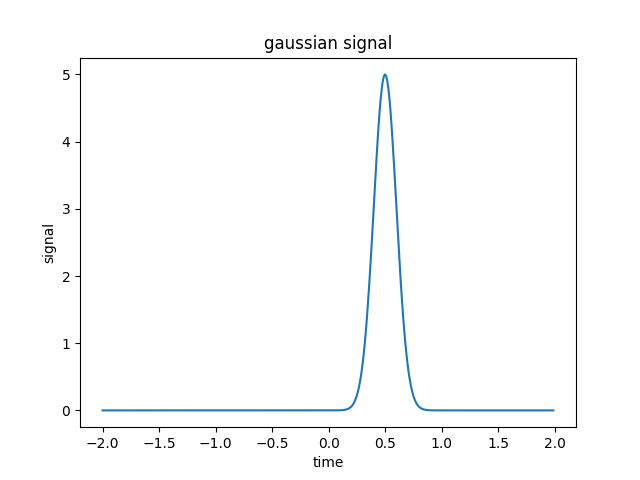
\includegraphics[width=0.75\textwidth]{plots/gauss_signal.png}
\caption{\label{fig:gauss_signal}  }
\end{figure}

\begin{figure}[h!]
\centering
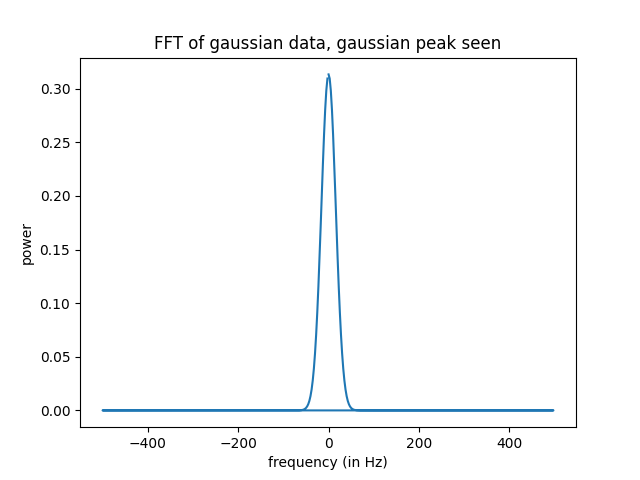
\includegraphics[width=0.75\textwidth]{plots/gauss_fft.png}
\caption{\label{fig:gauss_fft}  }
\end{figure}

\begin{figure}[h!]
\centering
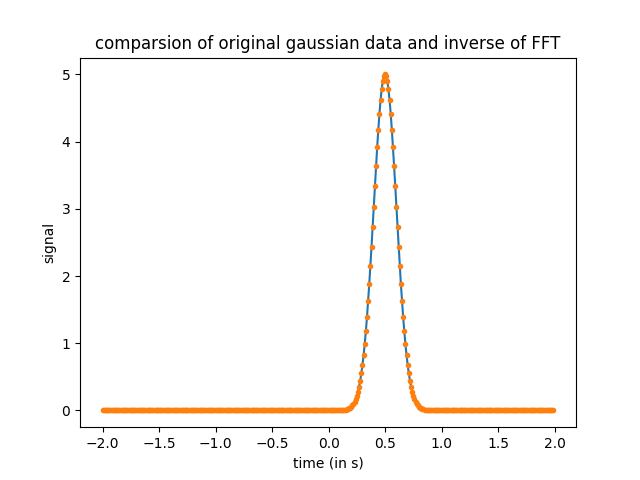
\includegraphics[width=0.75\textwidth]{plots/gauss_inverse.png}
\caption{\label{fig:gauss_inverse}  }
\end{figure}

\section{Arecibo (RIP, 1963 to 2020)}

\subsection{FFT on Arecibo data}

I imported the data given into Python using \texttt{open}. With sampling rate $1000$ (as each data point is separated by 1 millisecond), the data in time space is shown in \ref{fig:arecibo_time}. As expected, no clear signal can be seen.

\begin{figure}[h!]
\centering
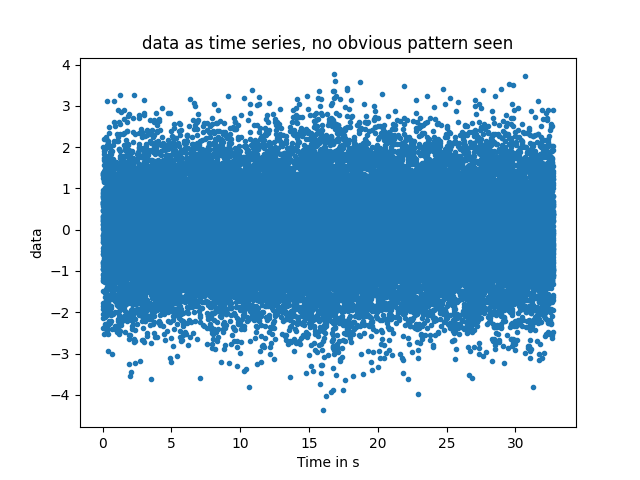
\includegraphics[width=0.75\textwidth]{plots/arecibo_time.png}
\caption{\label{fig:arecibo_time}  }
\end{figure}

Running the \texttt{scipy} FFT code again, we get Fig. \ref{fig:arecibo_freq}. Amongst all the noise, we see two high peaks! The two peaks are at $f ~ \pm 137$ Hz. So, the frequency of the signal is $137$ Hz.

\begin{figure}[h!]
\centering
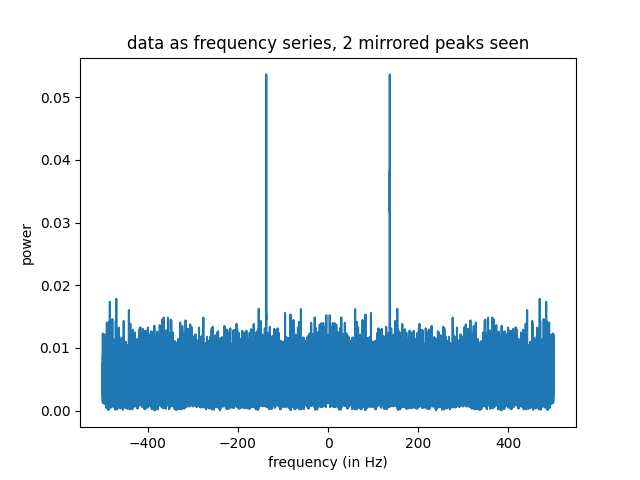
\includegraphics[width=0.75\textwidth]{plots/arecibo_freq.png}
\caption{\label{fig:arecibo_freq}  }
\end{figure}

Zooming into the peaks as in \ref{fig:arecibo_freq_zoom}, we see that the peak is not exactly sharp, but rather it is similar to a Gaussian, as expected for part (b).

\begin{figure}[h!]
\centering
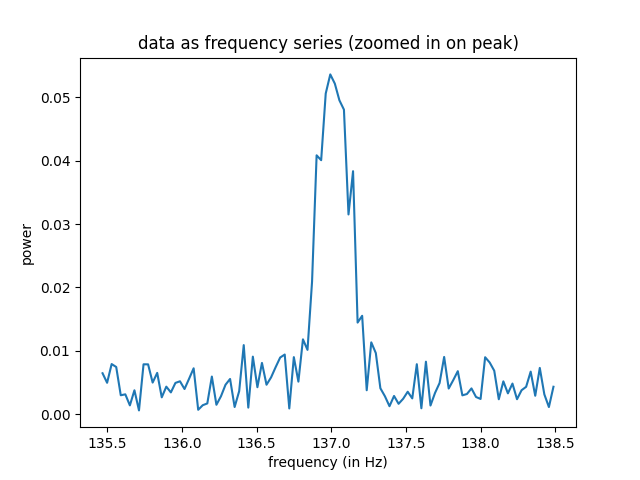
\includegraphics[width=0.75\textwidth]{plots/arecibo_freq_zoom.png}
\caption{\label{fig:arecibo_freq_zoom}  }
\end{figure}

\subsection{Gaussian Envelope}

I wrote the function \texttt{gaussian_sinusoidal} that returns a sinusoidal signal that has been modulated by a gaussian envelope. Examples for how the signal looks for $\Delta t=1$ and frequency $f=10$ Hz or $f=137$ Hz are shown in \ref{fig:arecibo_gauss_sim} and \ref{fig:arecibo_gauss_sim137} respectively. The FFT of the latter data set for $\Delta t=1$ and $f=137$ is seen in \ref{fig:arecibo_dT1}

\begin{figure}[h!]
\centering
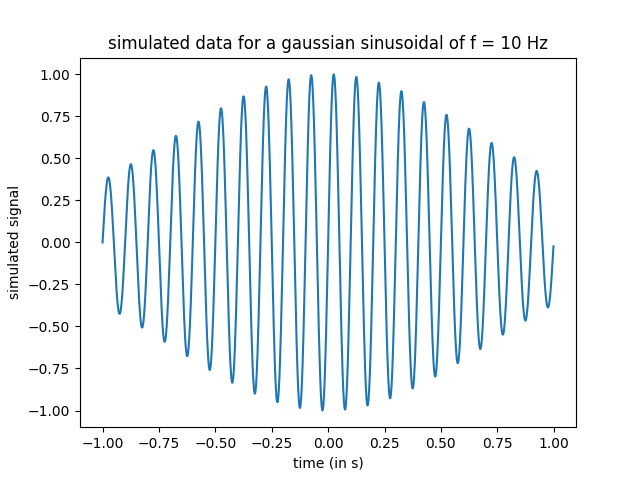
\includegraphics[width=0.75\textwidth]{plots/arecibo_gauss_sim.png}
\caption{\label{fig:arecibo_gauss_sim}  }
\end{figure}


\begin{figure}[h!]
\centering
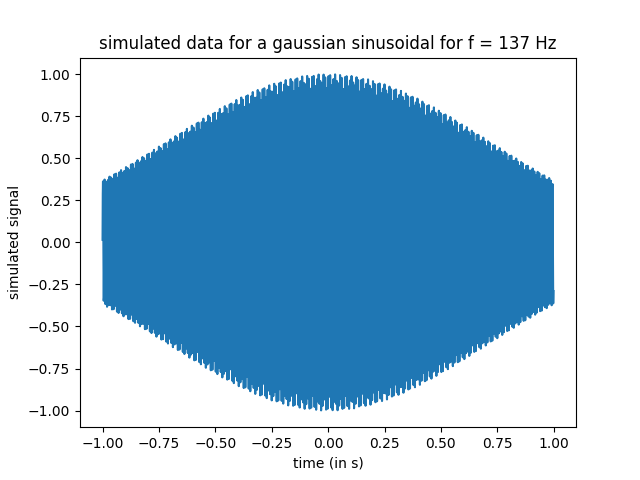
\includegraphics[width=0.75\textwidth]{plots/arecibo_gauss_sim137.png}
\caption{\label{fig:arecibo_gauss_sim137}  }
\end{figure}

\begin{figure}[h!]
\centering
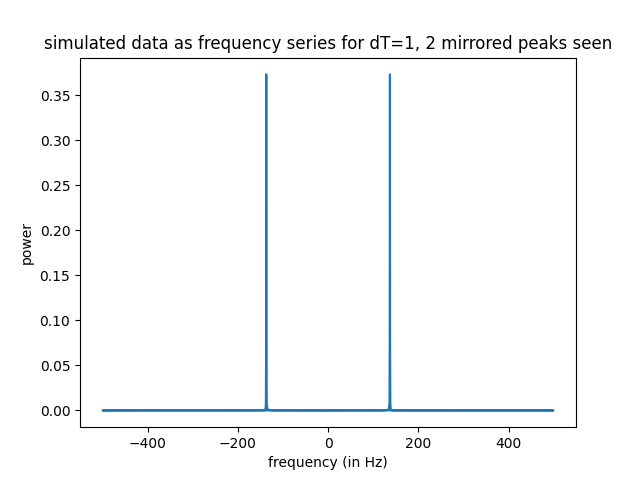
\includegraphics[width=0.75\textwidth]{plots/arecibo_dT1.png}
\caption{\label{fig:arecibo_dT1}  }
\end{figure}

Now, I automated this process for several values of $\Delta t$ to get a overlaid plot as in Fig. \ref{fig:arecibo_dTs}. Comparing to the original data FFT, we note that the actual value of $\Delta t \approx 2$. Running this process again for values closer to 2, we get Fig. \ref{fig:arecibo_dTs2}. It looks like $\Delta t \approx 1.9$ works best, but it is tough to tell. We can probably run a real curve-fitting routine to figure this out (like \texttt{scipy.optimize.curve_fit}).

\begin{figure}[h!]
\centering
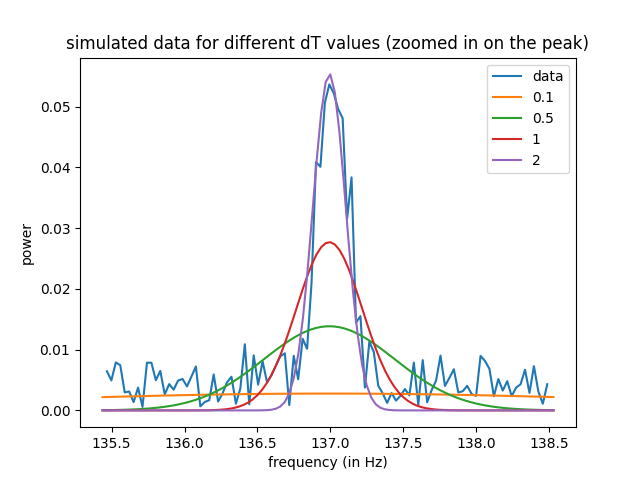
\includegraphics[width=0.75\textwidth]{plots/arecibo_dTs.png}
\caption{\label{fig:arecibo_dTs}  }
\end{figure}

\begin{figure}[h!]
\centering
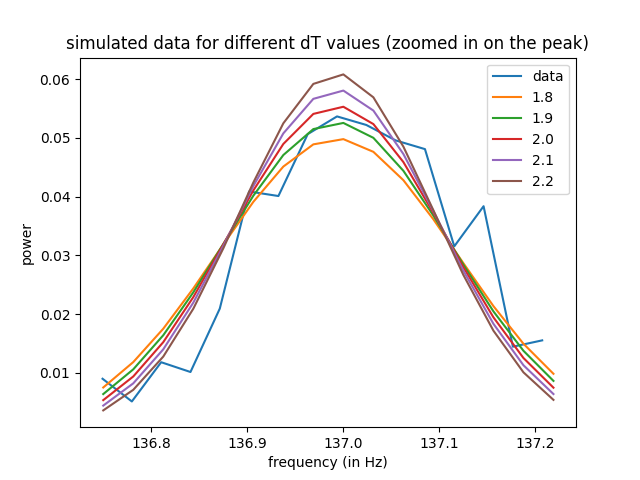
\includegraphics[width=0.75\textwidth]{plots/arecibo_dTs2.png}
\caption{\label{fig:arecibo_dTs2}  }
\end{figure}


\section{Unequally Sampled Data}

\subsection{Python Lomb-Scargle}

I decided to use \texttt{astropy.timeseries.LombScargle}.

\subsection{Gaussian and Arecibo using Lomb-Scargle}

Output of the Lomb Scargle algorithm on the Gaussian and Arecibo data is shown in Figs. \ref{fig:gauss_LombScargle} and \ref{fig:arecibo_LombScargle}. These looks like what we expected; the Gaussian transform is again Gaussian (and more noise because we restrict our frequency range). The Arecibo data has a peak at 137 Hz again.

\begin{figure}[h!]
\centering
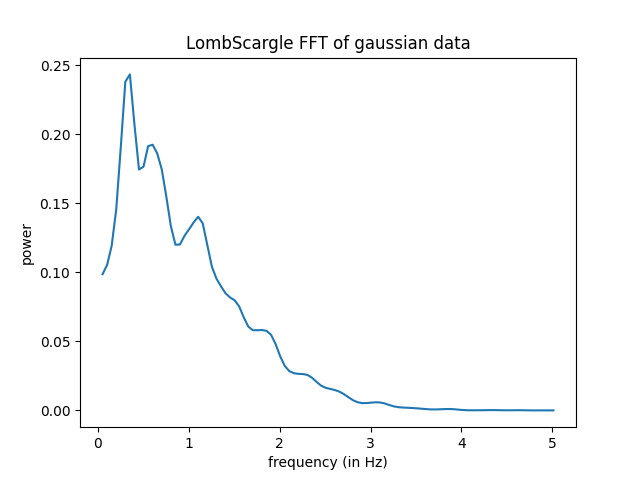
\includegraphics[width=0.75\textwidth]{plots/gauss_LombScargle.png}
\caption{\label{fig:gauss_LombScargle}  }
\end{figure}

\begin{figure}[h!]
\centering
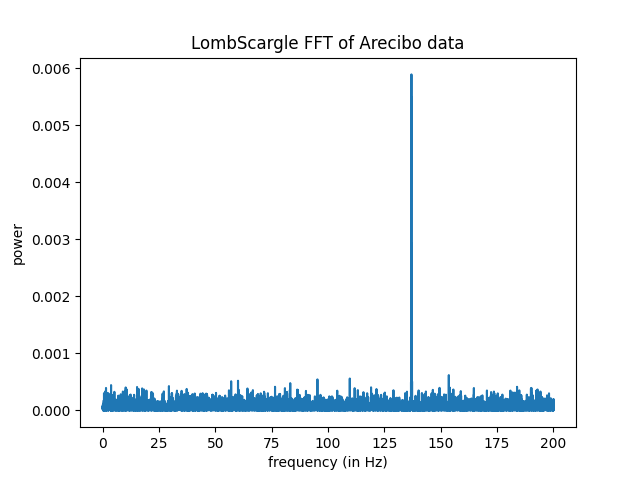
\includegraphics[width=0.75\textwidth]{plots/arecibo_LombScargle.png}
\caption{\label{fig:arecibo_LombScargle}  }
\end{figure}

\subsection{ZTF data}

We ran the same code on the ZFT data for Her X-1, obtained using the lab1 code. Fig. \ref{fig:ZFT_LombScargle} shows the result, with the period 1.70 days plotted as a orange dotted line. We do see a peak at the expected period, but there are other significant peaks too. Reasons for these might include the electronics used to obtain data. There can also be fake periods introduced due to the restrictions on data taking from a signal location on Earth. 

\begin{figure}[h!]
\centering
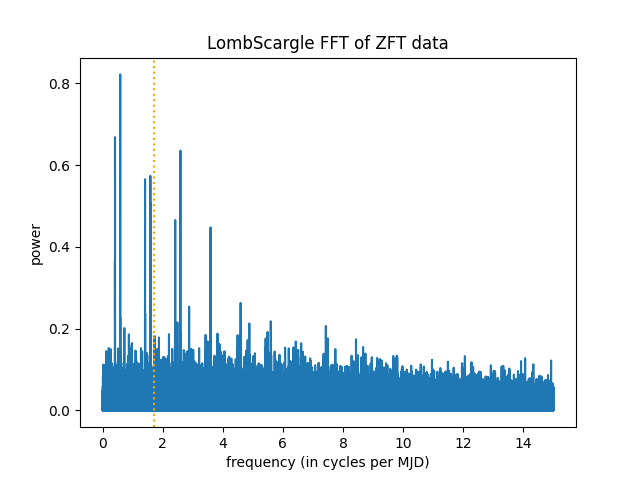
\includegraphics[width=0.75\textwidth]{plots/ZFT_LombScargle.png}
\caption{\label{fig:ZFT_LombScargle}  }
\end{figure}
\end{document}